%!TEX root = ../RfCPN.tex


\modHeadchapter[lof]{加工システムの全体の流れ}



%%%%%%%%%%%%%%%%%%%%%%%%%%%%%%%%%%%%%%%%%%%%%%%%%%%%%%%%%%
%% section 06.01 %%%%%%%%%%%%%%%%%%%%%%%%%%%%%%%%%%%%%%%%%
%%%%%%%%%%%%%%%%%%%%%%%%%%%%%%%%%%%%%%%%%%%%%%%%%%%%%%%%%%
\modHeadsection{加工全体の流れ}
加工全体の流れは\pageautoref{sec:MillingSystemFlow}に基づく。


%%%%%%%%%%%%%%%%%%%%%%%%%%%%%%%%%%%%%%%%%%%%%%%%%%%%%%%%%%
%% subsection 06.02.01 %%%%%%%%%%%%%%%%%%%%%%%%%%%%%%%%%%%
%%%%%%%%%%%%%%%%%%%%%%%%%%%%%%%%%%%%%%%%%%%%%%%%%%%%%%%%%%
\subsection{工程:加工前の段取}
\begin{enumerate}[label*=\sarrow]
\item ワークを\Table 上の専用\Jig に取り付ける
\item \Palette を交換し、ワークを機内に搬入する
\end{enumerate}


%%%%%%%%%%%%%%%%%%%%%%%%%%%%%%%%%%%%%%%%%%%%%%%%%%%%%%%%%%
%% figure %%%%%%%%%%%%%%%%%%%%%%%%%%%%%%%%%%%%%%%%%%%%%%%%
%%%%%%%%%%%%%%%%%%%%%%%%%%%%%%%%%%%%%%%%%%%%%%%%%%%%%%%%%%
\begin{figure}[h]%
\begin{FigShortbox}[valign=top]%
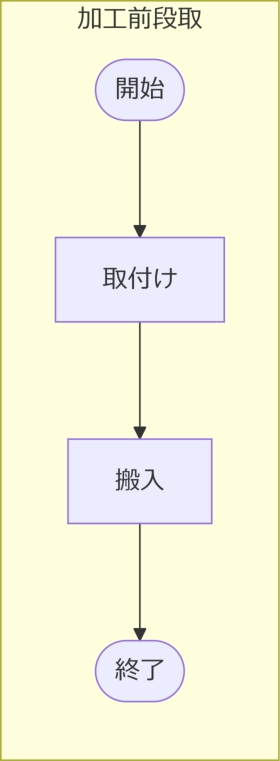
\includegraphics{RfCPN_p03_pictures/Pre_processing_Preparation_flow_chart.pdf}%
\setlength{\abovecaptionskip}{10pt}%
\captionof{figure}{加工前段取のフロー(概要)}
\end{FigShortbox}%
\end{figure}%
%%%%%%%%%%%%%%%%%%%%%%%%%%%%%%%%%%%%%%%%%%%%%%%%%%%%%%%%%%
%%%%%%%%%%%%%%%%%%%%%%%%%%%%%%%%%%%%%%%%%%%%%%%%%%%%%%%%%%
%%%%%%%%%%%%%%%%%%%%%%%%%%%%%%%%%%%%%%%%%%%%%%%%%%%%%%%%%%


\clearpage
%%%%%%%%%%%%%%%%%%%%%%%%%%%%%%%%%%%%%%%%%%%%%%%%%%%%%%%%%%
%% subsection 06.02.02 %%%%%%%%%%%%%%%%%%%%%%%%%%%%%%%%%%%
%%%%%%%%%%%%%%%%%%%%%%%%%%%%%%%%%%%%%%%%%%%%%%%%%%%%%%%%%%
\subsection{工程:加工前の測定}

%%%%%%%%%%%%%%%%%%%%%%%%%%%%%%%%%%%%%%%%%%%%%%%%%%%%%%%%%%
%% subsubsection 06.02.02.1 %%%%%%%%%%%%%%%%%%%%%%%%%%%%%%
%%%%%%%%%%%%%%%%%%%%%%%%%%%%%%%%%%%%%%%%%%%%%%%%%%%%%%%%%%
\subsubsection{ワーク座標系原点設定(ボトム側)}
\begin{enumerate}[label*=\sarrow]
\item ボトム側が工具側になるよう回転する
\item \BottomEndFace 部の外側中心を測定する
\item \BottomEndFace 部の内側中心を測定する
\end{enumerate}


%%%%%%%%%%%%%%%%%%%%%%%%%%%%%%%%%%%%%%%%%%%%%%%%%%%%%%%%%%
%% figure %%%%%%%%%%%%%%%%%%%%%%%%%%%%%%%%%%%%%%%%%%%%%%%%
%%%%%%%%%%%%%%%%%%%%%%%%%%%%%%%%%%%%%%%%%%%%%%%%%%%%%%%%%%
\begin{figure}[h]%
\begin{Figbox}[valign=top]%
\resizebox{\linewidth-35pt}{!}{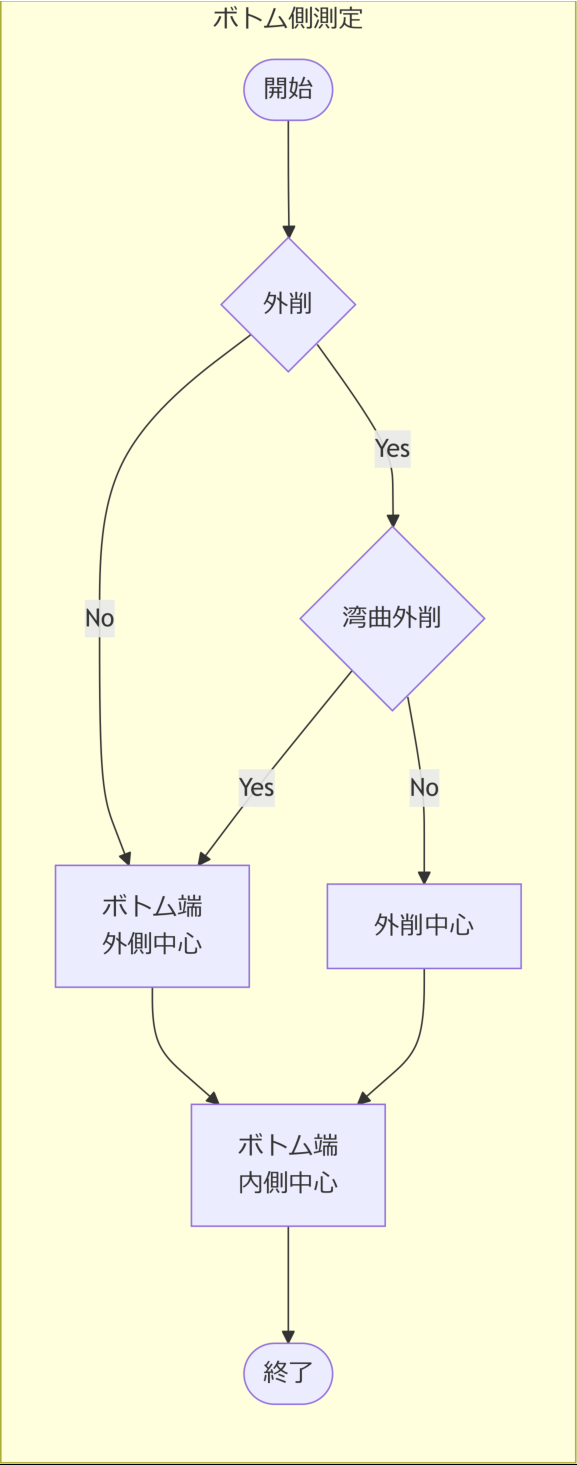
\includegraphics{RfCPN_p03_pictures/Pre_processing_Measurement_bot_flow_chart.pdf}}%
\setlength{\abovecaptionskip}{10pt}%
\captionof{figure}{加工前の測定のフロー(概要)}%\label{fig:mouldwithukeita}
\end{Figbox}%
\end{figure}%
%%%%%%%%%%%%%%%%%%%%%%%%%%%%%%%%%%%%%%%%%%%%%%%%%%%%%%%%%%
%%%%%%%%%%%%%%%%%%%%%%%%%%%%%%%%%%%%%%%%%%%%%%%%%%%%%%%%%%
%%%%%%%%%%%%%%%%%%%%%%%%%%%%%%%%%%%%%%%%%%%%%%%%%%%%%%%%%%


%%%%%%%%%%%%%%%%%%%%%%%%%%%%%%%%%%%%%%%%%%%%%%%%%%%%%%%%%%
%% subsubsection 06.02.02.2 %%%%%%%%%%%%%%%%%%%%%%%%%%%%%%
%%%%%%%%%%%%%%%%%%%%%%%%%%%%%%%%%%%%%%%%%%%%%%%%%%%%%%%%%%
\subsubsection{ワーク座標系原点設定(トップ側)}
\begin{enumerate}[label*=\sarrow]
\item トップ側が工具側になるよう回転する
\item \TopEndFace 部の外側中心を測定する
\item \TopEndFace 部の内側中心を測定する
\item \KeywayCenter を測定する
\end{enumerate}

%%%%%%%%%%%%%%%%%%%%%%%%%%%%%%%%%%%%%%%%%%%%%%%%%%%%%%%%%%
%% subsubsection 06.02.02.3 %%%%%%%%%%%%%%%%%%%%%%%%%%%%%%
%%%%%%%%%%%%%%%%%%%%%%%%%%%%%%%%%%%%%%%%%%%%%%%%%%%%%%%%%%
\subsubsection{\DimpleMeasurement}
\begin{enumerate}[label*=\sarrow]
\item すべての\Dimple の表面位置を測定する
\end{enumerate}


%%%%%%%%%%%%%%%%%%%%%%%%%%%%%%%%%%%%%%%%%%%%%%%%%%%%%%%%%%
%% subsection 06.02.03 %%%%%%%%%%%%%%%%%%%%%%%%%%%%%%%%%%%
%%%%%%%%%%%%%%%%%%%%%%%%%%%%%%%%%%%%%%%%%%%%%%%%%%%%%%%%%%
\subsection{工程:トップ側の加工}
\begin{enumerate}[label*=\sarrow]
\item \DimpleMilling を行う
\item \TopEndFacecutMilling を行う
\item (存在する場合)\TopOutcutMilling を行う
\item (存在する場合)\TopCurvedOutcutMilling を行う
\item (存在する場合)\EndFaceBoringMilling を行う
\item (存在する場合)\IncutBoringMilling を行う
\item \TopEndFaceOutCChamferMilling を行う
\item \TopEndFaceInCChamferMilling を行う
\end{enumerate}


\clearpage
%%%%%%%%%%%%%%%%%%%%%%%%%%%%%%%%%%%%%%%%%%%%%%%%%%%%%%%%%%
%% subsection 06.02.04 %%%%%%%%%%%%%%%%%%%%%%%%%%%%%%%%%%%
%%%%%%%%%%%%%%%%%%%%%%%%%%%%%%%%%%%%%%%%%%%%%%%%%%%%%%%%%%
\subsection{工程:ボトム側の加工}
\begin{enumerate}[label*=\sarrow]
\item ボトム側が工具側になるよう回転する
\item \BottomEndFacecutMilling を行う
\item (存在する場合)\BottomOutcutMilling を行う
\item (存在する場合)\BottomCurvedOutcutMilling を行う
\item \BottomEndFaceOutCChamferMilling を行う
\item \BottomEndFaceInCChamferMilling を行う
\end{enumerate}


%%%%%%%%%%%%%%%%%%%%%%%%%%%%%%%%%%%%%%%%%%%%%%%%%%%%%%%%%%
%% subsection 06.02.05 %%%%%%%%%%%%%%%%%%%%%%%%%%%%%%%%%%%
%%%%%%%%%%%%%%%%%%%%%%%%%%%%%%%%%%%%%%%%%%%%%%%%%%%%%%%%%%
\subsection{工程:加工後の測定}
\begin{enumerate}[label*=\sarrow]
\item \TopOutcut と\BottomOutcut の両方が存在する場合、\CenterlineEndFaceDifMeasurement を行う
\end{enumerate}


%%%%%%%%%%%%%%%%%%%%%%%%%%%%%%%%%%%%%%%%%%%%%%%%%%%%%%%%%%
%% subsection 41.01.06 %%%%%%%%%%%%%%%%%%%%%%%%%%%%%%%%%%%
%%%%%%%%%%%%%%%%%%%%%%%%%%%%%%%%%%%%%%%%%%%%%%%%%%%%%%%%%%
\subsection{工程:加工後の段取}
\begin{enumerate}[label*=\sarrow]
\item \Palette を交換し、ワークを機外に搬出する
\item ワークを\Table 上の専用\Jig から取り外す
\end{enumerate}


%%%%%%%%%%%%%%%%%%%%%%%%%%%%%%%%%%%%%%%%%%%%%%%%%%%%%%%%%%
%% figure %%%%%%%%%%%%%%%%%%%%%%%%%%%%%%%%%%%%%%%%%%%%%%%%
%%%%%%%%%%%%%%%%%%%%%%%%%%%%%%%%%%%%%%%%%%%%%%%%%%%%%%%%%%
\begin{figure}[p]%
\begin{Figlandscape}
\begin{adjustbox}{%
  addcode={\begin{minipage}{\textheight}\centering}{%
    \captionof{figure}{加工全体のフロー(概要):加工~加工後段取\label{fig:flowchartSecond}}%
    \end{minipage}%
  },
  rotate=90,
  center,
%  max width=\textheight,
%  max height=\linewidth,
  keepaspectratio}
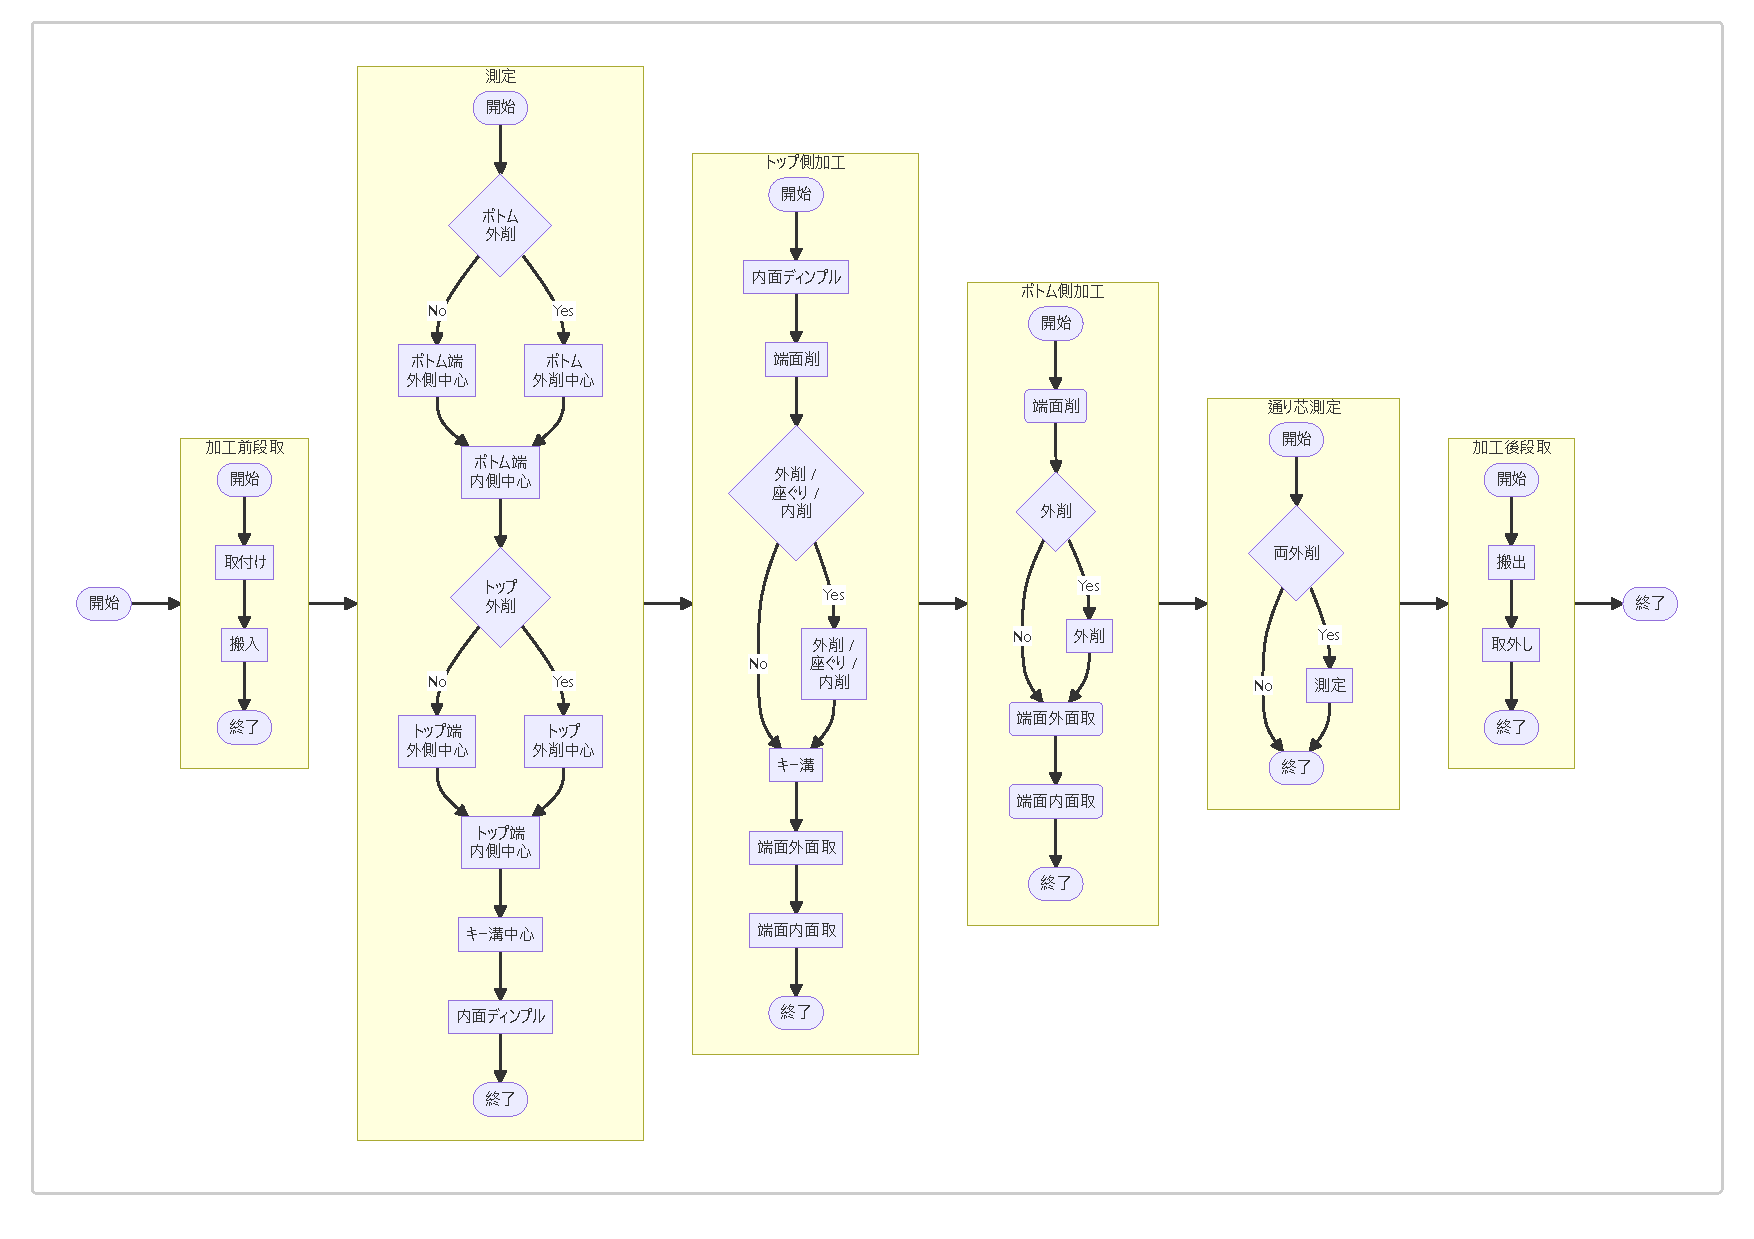
\includegraphics[height=\linewidth-10pt, trim=0 205 0 20, clip]{RfCPN_p03_pictures/Milling_flow_chart.pdf}%
\end{adjustbox}
\end{Figlandscape}%
\end{figure}%
%%%%%%%%%%%%%%%%%%%%%%%%%%%%%%%%%%%%%%%%%%%%%%%%%%%%%%%%%%
%%%%%%%%%%%%%%%%%%%%%%%%%%%%%%%%%%%%%%%%%%%%%%%%%%%%%%%%%%
%%%%%%%%%%%%%%%%%%%%%%%%%%%%%%%%%%%%%%%%%%%%%%%%%%%%%%%%%%


